\documentclass[slide]{../../custom}

\begin{document}

\begin{frame}
  \titlepage
\end{frame}

\begin{frame}
  \frametitle{摘要}
  \begin{itemize}
    \item \textbf{实现进展}:完成SPHINCS\textsuperscript{+}算法签名实现
    \item \textbf{分析工作}:研究签名过程的时间复杂度,确定优化方向
  \end{itemize}
\end{frame}

\begin{frame}
  \frametitle{FORS实现}
  \begin{itemize}
    \item 将$8 \times n$比特长度的$hm$分割成$k$份
    \item 构建$k$棵子树,每棵高度为$t$
    \item 计算每棵子树的根节点和认证路径
  \end{itemize}

  \begin{figure}[h]
    \centering
    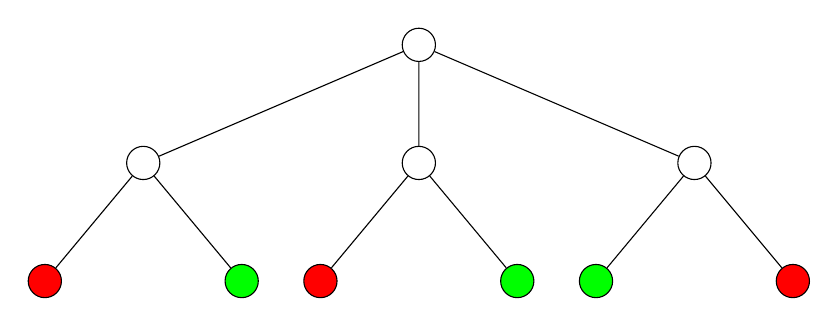
\begin{tikzpicture}[level distance=1.5cm,
        level 1/.style={sibling distance=3.5cm},
        level 2/.style={sibling distance=2.5cm},
      every node/.style={circle, draw, fill=white, inner sep=4pt, minimum size=12pt}]
      \node (root) [] {}
      child {node [] {}
        child {node [fill=red!100] {}}
        child {node [fill=green!100] {}}
      }
      child {node [] {}
        child {node [fill=red!100] {}}
        child {node [fill=green!100] {}}
      }
      child {node [] {}
        child {node [fill=green!100] {}}
        child {node [fill=red!100] {}}
      };
    \end{tikzpicture}
    \caption{FORS树示例 ($k=3,t=1$)}
  \end{figure}
\end{frame}

\begin{frame}
  \frametitle{HT树实现}
  \begin{itemize}
    \item $d$层Merkle树结构
    \item 每层使用WOTS+签名计算
    \item 最终生成公钥根节点
  \end{itemize}

  \begin{figure}
    \centering
    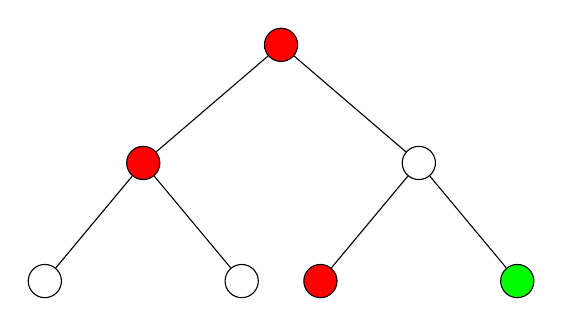
\begin{tikzpicture}[level distance=1.5cm,
        level 1/.style={sibling distance=3.5cm},
        level 2/.style={sibling distance=2.5cm},
      every node/.style={circle, draw, fill=white, inner sep=4pt, minimum size=12pt}]
      \node (root) [fill=red!100] {}
      child {node [fill=red!100] {}
        child {node [] {}}
        child {node [] {}}
      }
      child {node [] {}
        child {node [fill=red!100] {}}
        child {node [fill=green!100] {}}
      };
    \end{tikzpicture}
    \caption{HT树示例 ($h'=1,d=2$)}
  \end{figure}
\end{frame}

\begin{frame}
  \frametitle{时间复杂度分析}
  \textbf{FORS阶段}:
  \begin{itemize}
    \item 叶子节点生成:$2^t k$次哈希
    \item 根节点计算:$2^t k + 1$次哈希
    \item 总计约$16n + 1$次哈希运算
  \end{itemize}

  \textbf{HT阶段}:
  \begin{itemize}
    \item WOTS+签名:$n w / \log w$次哈希/链
    \item 每层XMSS树:$2^{h'} (nw/\log{w} + 1)$次哈希
    \item 总计约$d \times 2^{h'} (\frac{n w}{\log w} + 1)$次哈希
  \end{itemize}
\end{frame}

\begin{frame}
  \frametitle{优化方向}
  \begin{itemize}
    \item \textbf{并行化重点}:HT树计算(占主要计算量)
    \item \textbf{具体策略}:
      \begin{itemize}
        \item FORS的$k$棵子树并行计算
        \item HT树$d$层XMSS树的并行计算
      \end{itemize}
    \item \textbf{预期效果}:在SPX-128f配置($k=33, d=22$)下显著提升性能
  \end{itemize}
\end{frame}

\begin{frame}
  \frametitle{老师评语}
  \begin{alertblock}{你是对比哪个档次期刊来做这个工作的,参考对比决定了你将来发论文的档次}
    IEEE transaction of Compute 2024 《CUSPX: Efficient GPU Implementations of Post-Quantum Signature SPHINCS+》
  \end{alertblock}
  \begin{block}{下周计划}
    \begin{itemize}
      \item GPU并行化实现FORS和HT树
      \item 推进论文写作
    \end{itemize}
  \end{block}
\end{frame}

\end{document}
